% Options for packages loaded elsewhere
% Options for packages loaded elsewhere
\PassOptionsToPackage{unicode}{hyperref}
\PassOptionsToPackage{hyphens}{url}
\PassOptionsToPackage{dvipsnames,svgnames,x11names}{xcolor}
%
\documentclass[
  spanish,
  letterpaper,
  DIV=11,
  numbers=noendperiod]{scrartcl}
\usepackage{xcolor}
\usepackage[margin=2cm]{geometry}
\usepackage{amsmath,amssymb}
\setcounter{secnumdepth}{5}
\usepackage{iftex}
\ifPDFTeX
  \usepackage[T1]{fontenc}
  \usepackage[utf8]{inputenc}
  \usepackage{textcomp} % provide euro and other symbols
\else % if luatex or xetex
  \usepackage{unicode-math} % this also loads fontspec
  \defaultfontfeatures{Scale=MatchLowercase}
  \defaultfontfeatures[\rmfamily]{Ligatures=TeX,Scale=1}
\fi
\usepackage{lmodern}
\ifPDFTeX\else
  % xetex/luatex font selection
\fi
% Use upquote if available, for straight quotes in verbatim environments
\IfFileExists{upquote.sty}{\usepackage{upquote}}{}
\IfFileExists{microtype.sty}{% use microtype if available
  \usepackage[]{microtype}
  \UseMicrotypeSet[protrusion]{basicmath} % disable protrusion for tt fonts
}{}
\makeatletter
\@ifundefined{KOMAClassName}{% if non-KOMA class
  \IfFileExists{parskip.sty}{%
    \usepackage{parskip}
  }{% else
    \setlength{\parindent}{0pt}
    \setlength{\parskip}{6pt plus 2pt minus 1pt}}
}{% if KOMA class
  \KOMAoptions{parskip=half}}
\makeatother
% Make \paragraph and \subparagraph free-standing
\makeatletter
\ifx\paragraph\undefined\else
  \let\oldparagraph\paragraph
  \renewcommand{\paragraph}{
    \@ifstar
      \xxxParagraphStar
      \xxxParagraphNoStar
  }
  \newcommand{\xxxParagraphStar}[1]{\oldparagraph*{#1}\mbox{}}
  \newcommand{\xxxParagraphNoStar}[1]{\oldparagraph{#1}\mbox{}}
\fi
\ifx\subparagraph\undefined\else
  \let\oldsubparagraph\subparagraph
  \renewcommand{\subparagraph}{
    \@ifstar
      \xxxSubParagraphStar
      \xxxSubParagraphNoStar
  }
  \newcommand{\xxxSubParagraphStar}[1]{\oldsubparagraph*{#1}\mbox{}}
  \newcommand{\xxxSubParagraphNoStar}[1]{\oldsubparagraph{#1}\mbox{}}
\fi
\makeatother

\usepackage{color}
\usepackage{fancyvrb}
\newcommand{\VerbBar}{|}
\newcommand{\VERB}{\Verb[commandchars=\\\{\}]}
\DefineVerbatimEnvironment{Highlighting}{Verbatim}{commandchars=\\\{\}}
% Add ',fontsize=\small' for more characters per line
\usepackage{framed}
\definecolor{shadecolor}{RGB}{241,243,245}
\newenvironment{Shaded}{\begin{snugshade}}{\end{snugshade}}
\newcommand{\AlertTok}[1]{\textcolor[rgb]{0.68,0.00,0.00}{#1}}
\newcommand{\AnnotationTok}[1]{\textcolor[rgb]{0.37,0.37,0.37}{#1}}
\newcommand{\AttributeTok}[1]{\textcolor[rgb]{0.40,0.45,0.13}{#1}}
\newcommand{\BaseNTok}[1]{\textcolor[rgb]{0.68,0.00,0.00}{#1}}
\newcommand{\BuiltInTok}[1]{\textcolor[rgb]{0.00,0.23,0.31}{#1}}
\newcommand{\CharTok}[1]{\textcolor[rgb]{0.13,0.47,0.30}{#1}}
\newcommand{\CommentTok}[1]{\textcolor[rgb]{0.37,0.37,0.37}{#1}}
\newcommand{\CommentVarTok}[1]{\textcolor[rgb]{0.37,0.37,0.37}{\textit{#1}}}
\newcommand{\ConstantTok}[1]{\textcolor[rgb]{0.56,0.35,0.01}{#1}}
\newcommand{\ControlFlowTok}[1]{\textcolor[rgb]{0.00,0.23,0.31}{\textbf{#1}}}
\newcommand{\DataTypeTok}[1]{\textcolor[rgb]{0.68,0.00,0.00}{#1}}
\newcommand{\DecValTok}[1]{\textcolor[rgb]{0.68,0.00,0.00}{#1}}
\newcommand{\DocumentationTok}[1]{\textcolor[rgb]{0.37,0.37,0.37}{\textit{#1}}}
\newcommand{\ErrorTok}[1]{\textcolor[rgb]{0.68,0.00,0.00}{#1}}
\newcommand{\ExtensionTok}[1]{\textcolor[rgb]{0.00,0.23,0.31}{#1}}
\newcommand{\FloatTok}[1]{\textcolor[rgb]{0.68,0.00,0.00}{#1}}
\newcommand{\FunctionTok}[1]{\textcolor[rgb]{0.28,0.35,0.67}{#1}}
\newcommand{\ImportTok}[1]{\textcolor[rgb]{0.00,0.46,0.62}{#1}}
\newcommand{\InformationTok}[1]{\textcolor[rgb]{0.37,0.37,0.37}{#1}}
\newcommand{\KeywordTok}[1]{\textcolor[rgb]{0.00,0.23,0.31}{\textbf{#1}}}
\newcommand{\NormalTok}[1]{\textcolor[rgb]{0.00,0.23,0.31}{#1}}
\newcommand{\OperatorTok}[1]{\textcolor[rgb]{0.37,0.37,0.37}{#1}}
\newcommand{\OtherTok}[1]{\textcolor[rgb]{0.00,0.23,0.31}{#1}}
\newcommand{\PreprocessorTok}[1]{\textcolor[rgb]{0.68,0.00,0.00}{#1}}
\newcommand{\RegionMarkerTok}[1]{\textcolor[rgb]{0.00,0.23,0.31}{#1}}
\newcommand{\SpecialCharTok}[1]{\textcolor[rgb]{0.37,0.37,0.37}{#1}}
\newcommand{\SpecialStringTok}[1]{\textcolor[rgb]{0.13,0.47,0.30}{#1}}
\newcommand{\StringTok}[1]{\textcolor[rgb]{0.13,0.47,0.30}{#1}}
\newcommand{\VariableTok}[1]{\textcolor[rgb]{0.07,0.07,0.07}{#1}}
\newcommand{\VerbatimStringTok}[1]{\textcolor[rgb]{0.13,0.47,0.30}{#1}}
\newcommand{\WarningTok}[1]{\textcolor[rgb]{0.37,0.37,0.37}{\textit{#1}}}

\usepackage{longtable,booktabs,array}
\newcounter{none} % for unnumbered tables
\usepackage{calc} % for calculating minipage widths
% Correct order of tables after \paragraph or \subparagraph
\usepackage{etoolbox}
\makeatletter
\patchcmd\longtable{\par}{\if@noskipsec\mbox{}\fi\par}{}{}
\makeatother
% Allow footnotes in longtable head/foot
\IfFileExists{footnotehyper.sty}{\usepackage{footnotehyper}}{\usepackage{footnote}}
\makesavenoteenv{longtable}
\usepackage{graphicx}
\makeatletter
\newsavebox\pandoc@box
\newcommand*\pandocbounded[1]{% scales image to fit in text height/width
  \sbox\pandoc@box{#1}%
  \Gscale@div\@tempa{\textheight}{\dimexpr\ht\pandoc@box+\dp\pandoc@box\relax}%
  \Gscale@div\@tempb{\linewidth}{\wd\pandoc@box}%
  \ifdim\@tempb\p@<\@tempa\p@\let\@tempa\@tempb\fi% select the smaller of both
  \ifdim\@tempa\p@<\p@\scalebox{\@tempa}{\usebox\pandoc@box}%
  \else\usebox{\pandoc@box}%
  \fi%
}
% Set default figure placement to htbp
\def\fps@figure{htbp}
\makeatother



\ifLuaTeX
\usepackage[bidi=basic,shorthands=off,spanish,es-nodecimaldot,es-tabla]{babel}
\else
\usepackage[bidi=default,shorthands=off,spanish,es-nodecimaldot,es-tabla]{babel}
\fi
\ifLuaTeX
  \usepackage{selnolig} % disable illegal ligatures
\fi


\setlength{\emergencystretch}{3em} % prevent overfull lines

\providecommand{\tightlist}{%
  \setlength{\itemsep}{0pt}\setlength{\parskip}{0pt}}



 


% preamble.tex – Colegio Portaliano (para pdfLaTeX)

\usepackage[T1]{fontenc}
\usepackage[utf8]{inputenc}
\usepackage{lmodern}
\usepackage{newtxtext}
\usepackage[amsthm]{newtxmath}

% Caracteres Unicode problemáticos
\DeclareUnicodeCharacter{2248}{\ensuremath{\approx}}   % ≈
\DeclareUnicodeCharacter{22EE}{\ensuremath{\vdots}}    % ⋮
\DeclareUnicodeCharacter{22EF}{\ensuremath{\cdots}}    % ⋯
\DeclareUnicodeCharacter{22F1}{\ensuremath{\ddots}}    % ⋱

\AtBeginDocument{%
  \decimalpoint
  \deactivatequoting
}

\everymath{\displaystyle}
\KOMAoption{captions}{tableheading}
\makeatletter
\@ifpackageloaded{tcolorbox}{}{\usepackage[skins,breakable]{tcolorbox}}
\@ifpackageloaded{fontawesome5}{}{\usepackage{fontawesome5}}
\definecolor{quarto-callout-color}{HTML}{909090}
\definecolor{quarto-callout-note-color}{HTML}{0758E5}
\definecolor{quarto-callout-important-color}{HTML}{CC1914}
\definecolor{quarto-callout-warning-color}{HTML}{EB9113}
\definecolor{quarto-callout-tip-color}{HTML}{00A047}
\definecolor{quarto-callout-caution-color}{HTML}{FC5300}
\definecolor{quarto-callout-color-frame}{HTML}{acacac}
\definecolor{quarto-callout-note-color-frame}{HTML}{4582ec}
\definecolor{quarto-callout-important-color-frame}{HTML}{d9534f}
\definecolor{quarto-callout-warning-color-frame}{HTML}{f0ad4e}
\definecolor{quarto-callout-tip-color-frame}{HTML}{02b875}
\definecolor{quarto-callout-caution-color-frame}{HTML}{fd7e14}
\makeatother
\makeatletter
\@ifpackageloaded{caption}{}{\usepackage{caption}}
\AtBeginDocument{%
\ifdefined\contentsname
  \renewcommand*\contentsname{Tabla de contenidos}
\else
  \newcommand\contentsname{Tabla de contenidos}
\fi
\ifdefined\listfigurename
  \renewcommand*\listfigurename{Listado de Figuras}
\else
  \newcommand\listfigurename{Listado de Figuras}
\fi
\ifdefined\listtablename
  \renewcommand*\listtablename{Listado de Tablas}
\else
  \newcommand\listtablename{Listado de Tablas}
\fi
\ifdefined\figurename
  \renewcommand*\figurename{Figura}
\else
  \newcommand\figurename{Figura}
\fi
\ifdefined\tablename
  \renewcommand*\tablename{Tabla}
\else
  \newcommand\tablename{Tabla}
\fi
}
\@ifpackageloaded{float}{}{\usepackage{float}}
\floatstyle{ruled}
\@ifundefined{c@chapter}{\newfloat{codelisting}{h}{lop}}{\newfloat{codelisting}{h}{lop}[chapter]}
\floatname{codelisting}{Listado}
\newcommand*\listoflistings{\listof{codelisting}{Listado de Listados}}
\makeatother
\makeatletter
\makeatother
\makeatletter
\@ifpackageloaded{caption}{}{\usepackage{caption}}
\@ifpackageloaded{subcaption}{}{\usepackage{subcaption}}
\makeatother
\usepackage{bookmark}
\IfFileExists{xurl.sty}{\usepackage{xurl}}{} % add URL line breaks if available
\urlstyle{same}
\hypersetup{
  pdftitle={Lección 8: Introducción a la probabilidad},
  pdfauthor={Hans Sigrist},
  pdflang={es},
  colorlinks=true,
  linkcolor={blue},
  filecolor={Maroon},
  citecolor={Blue},
  urlcolor={Blue},
  pdfcreator={LaTeX via pandoc}}


\title{Lección 8: Introducción a la probabilidad}
\author{Hans Sigrist}
\date{2026-05-05}
\begin{document}
\maketitle
\begin{abstract}
Esta lección introduce la probabilidad como base de la inferencia
estadística. Se estudian conceptos como espacio muestral, probabilidad
de un evento, regla de la adición, complemento, independencia y
distribuciones de probabilidad. Mediante ejemplos con dados, cartas y
situaciones propias de la aviación (confiabilidad de motores,
cancelaciones de vuelo) se construye una comprensión operativa de la
probabilidad, apoyada en simulaciones con R.
\end{abstract}

\renewcommand*\contentsname{Tabla de contenidos}
{
\setcounter{tocdepth}{3}
\tableofcontents
}

\begin{figure}

\centering{

\pandocbounded{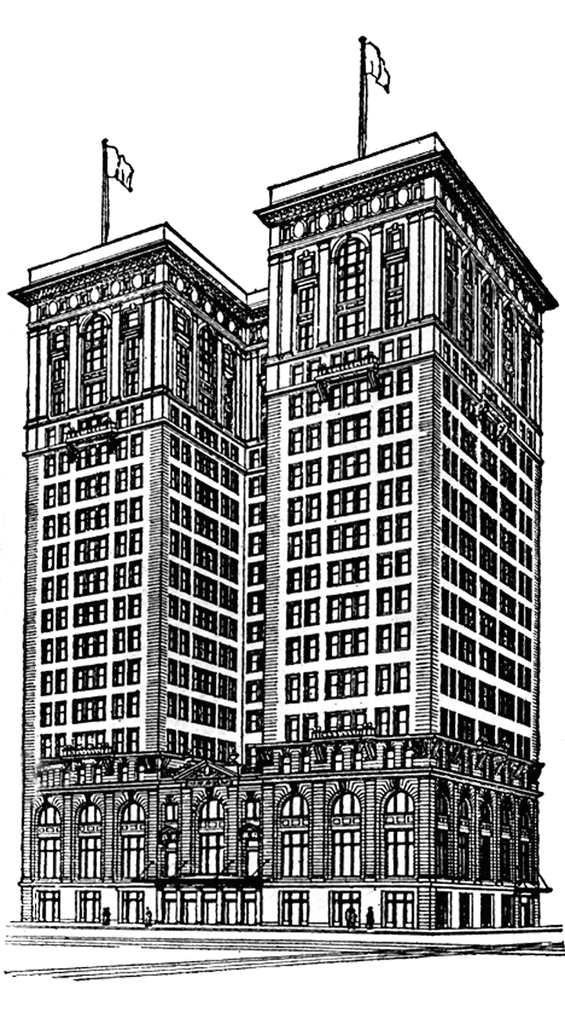
\includegraphics[keepaspectratio]{../imagenes/skyscraper_8098_lg.png}}

}

\caption{\label{fig-prob-cover-pdf}Vuelo 1549 de US Airways sobre el río
Hudson. La decisión del Capitán Sullenberger de amerizar fue el
resultado de una evaluación de riesgos ejecutada en segundos.}

\end{figure}%

\section{Objetivos de la lección}\label{objetivos-de-la-lecciuxf3n}

Al finalizar esta lección, serás capaz de:

\begin{itemize}
\tightlist
\item
  Definir \textbf{probabilidad} en su interpretación frecuentista y
  reconocer la \textbf{Ley de los Grandes Números}.
\item
  Describir un \textbf{espacio muestral} y calcular probabilidades de
  eventos sencillos.
\item
  Aplicar la \textbf{regla de la adición} para eventos disjuntos y la
  \textbf{regla general de la adición}.
\item
  Calcular la probabilidad del \textbf{complemento} de un evento y
  reconocer cuándo conviene usarlo.
\item
  Identificar eventos \textbf{independientes} y aplicar la \textbf{regla
  del producto}.
\item
  Construir e interpretar \textbf{distribuciones de probabilidad} para
  variables aleatorias discretas.
\item
  Usar R para simular experimentos aleatorios y verificar empíricamente
  las reglas teóricas.
\end{itemize}

\begin{center}\rule{0.5\linewidth}{0.5pt}\end{center}

\section{¿Qué es la probabilidad?}\label{quuxe9-es-la-probabilidad}

La probabilidad es la herramienta matemática que usamos para cuantificar
la incertidumbre. En estadística, actúa como puente entre la muestra y
la población: nos permite medir qué tan verosímil es una afirmación a
partir de los datos observados. Antes de estimar parámetros, contrastar
hipótesis o construir intervalos de confianza, necesitamos un lenguaje
preciso para hablar de lo incierto --- ese es, exactamente, el lenguaje
de la probabilidad.

\begin{tcolorbox}[enhanced jigsaw, arc=.35mm, bottomrule=.15mm, bottomtitle=1mm, breakable, colback=white, colbacktitle=quarto-callout-note-color!10!white, colframe=quarto-callout-note-color-frame, coltitle=black, left=2mm, leftrule=.75mm, opacityback=0, opacitybacktitle=0.6, rightrule=.15mm, title=\textcolor{quarto-callout-note-color}{\faInfo}\hspace{0.5em}{Definición: Probabilidad}, titlerule=0mm, toprule=.15mm, toptitle=1mm]

La \textbf{probabilidad} de un resultado es la proporción de veces que
dicho resultado ocurriría si observáramos el proceso aleatorio un número
infinito de veces. Es siempre un número en el intervalo \([0, 1]\): un
evento imposible tiene probabilidad \(0\) y un evento seguro tiene
probabilidad \(1\).

\end{tcolorbox}

Por ejemplo, si lanzamos un dado equilibrado, la probabilidad de obtener
un 1 es \(P(1) = 1/6 \approx 0{,}167\). Esto significa que, en una larga
serie de lanzamientos, aproximadamente el 16,7 \% arrojaría un 1.

\subsection{La Ley de los Grandes
Números}\label{la-ley-de-los-grandes-nuxfameros}

La probabilidad se manifiesta en la práctica mediante la \textbf{Ley de
los Grandes Números}: a medida que aumentamos el número de repeticiones,
la proporción observada \(\hat{p}_n\) de un resultado se acerca cada vez
más a su probabilidad teórica \(p\).

\begin{tcolorbox}[enhanced jigsaw, arc=.35mm, bottomrule=.15mm, bottomtitle=1mm, breakable, colback=white, colbacktitle=quarto-callout-note-color!10!white, colframe=quarto-callout-note-color-frame, coltitle=black, left=2mm, leftrule=.75mm, opacityback=0, opacitybacktitle=0.6, rightrule=.15mm, title=\textcolor{quarto-callout-note-color}{\faInfo}\hspace{0.5em}{Ley de los Grandes Números}, titlerule=0mm, toprule=.15mm, toptitle=1mm]

A medida que se recopilan más observaciones, la proporción \(\hat{p}_n\)
de ocurrencias con un resultado particular converge a la probabilidad
\(p\) de ese resultado.

\end{tcolorbox}

La siguiente simulación ilustra esta convergencia para el lanzamiento de
un dado justo, donde \(p = 1/6\).

\begin{Shaded}
\begin{Highlighting}[]
\FunctionTok{set.seed}\NormalTok{(}\DecValTok{123}\NormalTok{)}
\NormalTok{n }\OtherTok{\textless{}{-}} \DecValTok{100000}

\CommentTok{\# Simulamos n lanzamientos de un dado justo}
\NormalTok{lanzamientos }\OtherTok{\textless{}{-}} \FunctionTok{sample}\NormalTok{(}\DecValTok{1}\SpecialCharTok{:}\DecValTok{6}\NormalTok{, n, }\AttributeTok{replace =} \ConstantTok{TRUE}\NormalTok{)}

\CommentTok{\# Proporción acumulada de 1s tras cada lanzamiento}
\NormalTok{prop\_acum }\OtherTok{\textless{}{-}} \FunctionTok{cumsum}\NormalTok{(lanzamientos }\SpecialCharTok{==} \DecValTok{1}\NormalTok{) }\SpecialCharTok{/} \FunctionTok{seq\_along}\NormalTok{(lanzamientos)}

\CommentTok{\# Seleccionamos puntos para graficar más ágilmente}
\NormalTok{idx }\OtherTok{\textless{}{-}} \FunctionTok{unique}\NormalTok{(}\FunctionTok{c}\NormalTok{(}\DecValTok{1}\SpecialCharTok{:}\DecValTok{1000}\NormalTok{, }\FunctionTok{seq}\NormalTok{(}\DecValTok{1000}\NormalTok{, n, }\AttributeTok{by =} \DecValTok{200}\NormalTok{)))}

\FunctionTok{ggplot}\NormalTok{(}\FunctionTok{data.frame}\NormalTok{(}\AttributeTok{tiro =}\NormalTok{ idx, }\AttributeTok{prop =}\NormalTok{ prop\_acum[idx]),}
       \FunctionTok{aes}\NormalTok{(}\AttributeTok{x =}\NormalTok{ tiro, }\AttributeTok{y =}\NormalTok{ prop)) }\SpecialCharTok{+}
  \FunctionTok{geom\_line}\NormalTok{(}\AttributeTok{color =} \StringTok{"\#0758E5"}\NormalTok{, }\AttributeTok{linewidth =} \FloatTok{0.4}\NormalTok{) }\SpecialCharTok{+}
  \FunctionTok{geom\_hline}\NormalTok{(}\AttributeTok{yintercept =} \DecValTok{1}\SpecialCharTok{/}\DecValTok{6}\NormalTok{, }\AttributeTok{linetype =} \StringTok{"dashed"}\NormalTok{,}
             \AttributeTok{color =} \StringTok{"red"}\NormalTok{, }\AttributeTok{linewidth =} \FloatTok{0.9}\NormalTok{) }\SpecialCharTok{+}
  \FunctionTok{scale\_x\_continuous}\NormalTok{(}\AttributeTok{labels =}\NormalTok{ comma) }\SpecialCharTok{+}
  \FunctionTok{annotate}\NormalTok{(}\StringTok{"text"}\NormalTok{, }\AttributeTok{x =} \DecValTok{80000}\NormalTok{, }\AttributeTok{y =} \DecValTok{1}\SpecialCharTok{/}\DecValTok{6} \SpecialCharTok{+} \FloatTok{0.009}\NormalTok{,}
           \AttributeTok{label =} \StringTok{"p = 1/6"}\NormalTok{, }\AttributeTok{color =} \StringTok{"red"}\NormalTok{, }\AttributeTok{size =} \FloatTok{3.5}\NormalTok{) }\SpecialCharTok{+}
  \FunctionTok{labs}\NormalTok{(}\AttributeTok{x =} \StringTok{"Número de lanzamientos"}\NormalTok{,}
       \AttributeTok{y =} \FunctionTok{expression}\NormalTok{(}\FunctionTok{hat}\NormalTok{(p)[n]),}
       \AttributeTok{title =} \StringTok{"Convergencia de la proporción de 1s (Ley de los Grandes Números)"}\NormalTok{) }\SpecialCharTok{+}
  \FunctionTok{theme\_minimal}\NormalTok{(}\AttributeTok{base\_size =} \DecValTok{12}\NormalTok{)}
\end{Highlighting}
\end{Shaded}

\begin{figure}[H]

\centering{

\pandocbounded{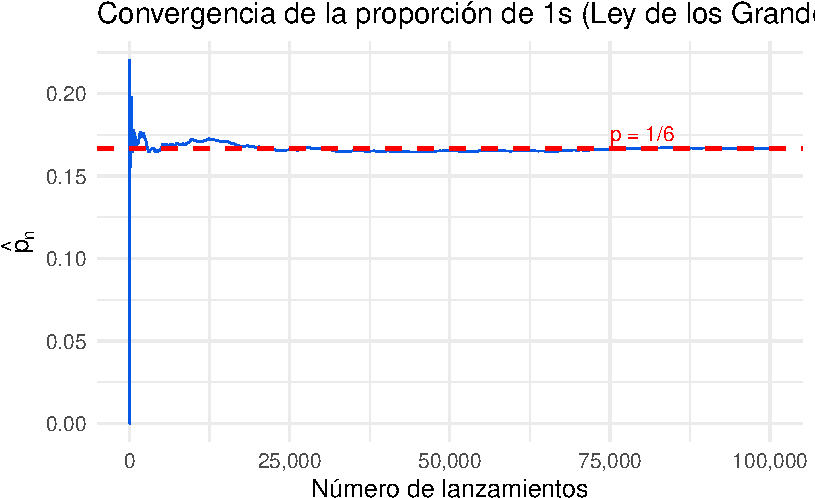
\includegraphics[keepaspectratio]{leccion-8-introduccion-a-la-probabilidad_files/figure-pdf/fig-lln-1.pdf}}

}

\caption{\label{fig-lln}Proporción acumulada de 1s al lanzar un dado
100.000 veces. La línea roja punteada indica la probabilidad teórica p =
1/6 ≈ 0,167. Las oscilaciones iniciales se amortiguan progresivamente.}

\end{figure}%

Nota que para pocas observaciones la proporción oscila
considerablemente. Esas oscilaciones no son una violación de la ley: son
exactamente lo que cabría esperar. La Ley de los Grandes Números
garantiza que las desviaciones se hacen progresivamente más pequeñas,
pero no que desaparezcan en ningún lanzamiento concreto.

\begin{center}\rule{0.5\linewidth}{0.5pt}\end{center}

\section{Espacio muestral y eventos}\label{espacio-muestral-y-eventos}

El \textbf{espacio muestral} \(S\) es el conjunto de todos los
resultados posibles de un experimento aleatorio. Un \textbf{evento} es
cualquier subconjunto del espacio muestral.

Al lanzar un dado, \(S = \{1, 2, 3, 4, 5, 6\}\), y el evento ``obtener
número par'' es \(A = \{2, 4, 6\}\). Al lanzar una moneda,
\(S = \{\text{Cara}, \text{Sello}\}\). En contexto aeronáutico, al
observar si un vuelo sale a tiempo,
\(S = \{\text{A tiempo}, \text{Demorado}\}\).

Escribimos \(P(A)\) para denotar la probabilidad del evento \(A\).
Cuando el espacio muestral tiene \(n\) resultados igualmente probables y
el evento \(A\) contiene \(k\) de ellos, entonces \(P(A) = k/n\).

\begin{center}\rule{0.5\linewidth}{0.5pt}\end{center}

\section{Eventos disjuntos y regla de la
adición}\label{eventos-disjuntos-y-regla-de-la-adiciuxf3n}

\subsection{Eventos mutuamente
excluyentes}\label{eventos-mutuamente-excluyentes}

Dos eventos son \textbf{disjuntos} (o \textbf{mutuamente excluyentes})
si no pueden ocurrir simultáneamente. Al lanzar un dado, ``sale 1'' y
``sale 2'' son disjuntos porque en un mismo lanzamiento sólo puede
ocurrir uno. En cambio, ``sale 1'' y ``sale número impar'' no son
disjuntos, pues ambos ocurren cuando el resultado es 1.

\begin{tcolorbox}[enhanced jigsaw, arc=.35mm, bottomrule=.15mm, bottomtitle=1mm, breakable, colback=white, colbacktitle=quarto-callout-important-color!10!white, colframe=quarto-callout-important-color-frame, coltitle=black, left=2mm, leftrule=.75mm, opacityback=0, opacitybacktitle=0.6, rightrule=.15mm, title=\textcolor{quarto-callout-important-color}{\faExclamation}\hspace{0.5em}{Regla de la adición para eventos disjuntos}, titlerule=0mm, toprule=.15mm, toptitle=1mm]

Si \(A_1\) y \(A_2\) son eventos disjuntos, entonces

\[P(A_1 \text{ o } A_2) = P(A_1) + P(A_2).\]

Más en general, para \(k\) eventos mutuamente excluyentes
\(A_1, \ldots, A_k\),

\[P(A_1 \text{ o } A_2 \text{ o } \cdots \text{ o } A_k) = \sum_{i=1}^{k} P(A_i).\]

\end{tcolorbox}

\textbf{Ejemplo aeronáutico.} Un aeropuerto registra las causas de
retraso. La probabilidad de que un vuelo se retrase por condiciones
meteorológicas es \(0{,}12\) y por falla mecánica es \(0{,}05\). Si
ambas causas son mutuamente excluyentes como causa principal del
retraso, entonces

\[P(\text{meteorología o falla}) = 0{,}12 + 0{,}05 = 0{,}17.\]

\subsection{Regla general de la
adición}\label{regla-general-de-la-adiciuxf3n}

Cuando los eventos no son disjuntos, la suma simple de probabilidades
cuenta dos veces los resultados en la intersección. La corrección da
lugar a la regla general.

\begin{tcolorbox}[enhanced jigsaw, arc=.35mm, bottomrule=.15mm, bottomtitle=1mm, breakable, colback=white, colbacktitle=quarto-callout-important-color!10!white, colframe=quarto-callout-important-color-frame, coltitle=black, left=2mm, leftrule=.75mm, opacityback=0, opacitybacktitle=0.6, rightrule=.15mm, title=\textcolor{quarto-callout-important-color}{\faExclamation}\hspace{0.5em}{Regla general de la adición}, titlerule=0mm, toprule=.15mm, toptitle=1mm]

Para cualesquiera dos eventos \(A\) y \(B\), disjuntos o no,

\[P(A \text{ o } B) = P(A) + P(B) - P(A \text{ y } B),\]

donde \(P(A \text{ y } B)\) es la probabilidad de que ocurran ambos
simultáneamente.

\end{tcolorbox}

\begin{tcolorbox}[enhanced jigsaw, arc=.35mm, bottomrule=.15mm, bottomtitle=1mm, breakable, colback=white, colbacktitle=quarto-callout-tip-color!10!white, colframe=quarto-callout-tip-color-frame, coltitle=black, left=2mm, leftrule=.75mm, opacityback=0, opacitybacktitle=0.6, rightrule=.15mm, title=\textcolor{quarto-callout-tip-color}{\faLightbulb}\hspace{0.5em}{«o» es inclusivo en estadística}, titlerule=0mm, toprule=.15mm, toptitle=1mm]

Cuando escribimos «\(A\) o \(B\)», queremos decir «\(A\), \(B\), o
ambos», salvo indicación en contrario.

\end{tcolorbox}

\textbf{Ejemplo con cartas.} En un mazo estándar de 52 cartas, sea \(A\)
= ``la carta es un diamante'' y \(B\) = ``la carta es una figura'' (J,
Q, K). Tenemos \(P(A) = 13/52\), \(P(B) = 12/52\) y
\(P(A \text{ y } B) = 3/52\) (las cartas J diamante, Q diamante, K
diamante pertenecen a ambos eventos). Entonces

\[P(A \text{ o } B) = \frac{13}{52} + \frac{12}{52} - \frac{3}{52} = \frac{22}{52} = \frac{11}{26} \approx 0{,}423.\]

\textbf{Ejemplo aeronáutico.} En cierto aeropuerto,
\(P(\text{cancelación por mal tiempo}) = 0{,}02\),
\(P(\text{cancelación por problemas técnicos}) = 0{,}01\), y
\(P(\text{ambas causas}) = 0{,}002\). Como no son disjuntos, aplicamos
la regla general:

\[P(\text{cancelación}) = 0{,}02 + 0{,}01 - 0{,}002 = 0{,}028.\]

\begin{center}\rule{0.5\linewidth}{0.5pt}\end{center}

\section{Complemento de un evento}\label{complemento-de-un-evento}

El \textbf{complemento} del evento \(A\), denotado \(A^c\), reúne todos
los resultados del espacio muestral que no pertenecen a \(A\). Por
construcción, \(A\) y \(A^c\) son disjuntos y juntos cubren todo \(S\),
de modo que \(P(A \text{ o } A^c) = 1\).

\begin{tcolorbox}[enhanced jigsaw, arc=.35mm, bottomrule=.15mm, bottomtitle=1mm, breakable, colback=white, colbacktitle=quarto-callout-important-color!10!white, colframe=quarto-callout-important-color-frame, coltitle=black, left=2mm, leftrule=.75mm, opacityback=0, opacitybacktitle=0.6, rightrule=.15mm, title=\textcolor{quarto-callout-important-color}{\faExclamation}\hspace{0.5em}{Regla del complemento}, titlerule=0mm, toprule=.15mm, toptitle=1mm]

\[P(A) + P(A^c) = 1, \qquad \text{es decir,} \qquad P(A) = 1 - P(A^c).\]

\end{tcolorbox}

Esta regla es especialmente valiosa cuando calcular \(P(A^c)\) es más
sencillo que calcular \(P(A)\) directamente. En problemas complejos, los
eventos del tipo ``al menos uno'' tienen como complemento natural
``ninguno'', y este suele ser mucho más fácil de calcular.

\textbf{Ejemplo.} Si la probabilidad de que un piloto apruebe un chequeo
médico es \(0{,}96\), la probabilidad de que no lo apruebe es
\(1 - 0{,}96 = 0{,}04\).

\textbf{Ejemplo con dados.} Al lanzar dos dados, la probabilidad de que
la suma sea menor que 12 resulta fácil de calcular por complemento: el
único resultado que produce suma exactamente 12 es (6, 6), con
probabilidad \(1/36\). Por tanto,

\[P(\text{suma} < 12) = 1 - P(\text{suma} = 12) = 1 - \frac{1}{36} = \frac{35}{36} \approx 0{,}972.\]

\begin{center}\rule{0.5\linewidth}{0.5pt}\end{center}

\section{Independencia y regla de la
multiplicación}\label{independencia-y-regla-de-la-multiplicaciuxf3n}

\subsection{Procesos independientes}\label{procesos-independientes}

Dos procesos son \textbf{independientes} si conocer el resultado de uno
no aporta información alguna sobre el resultado del otro. El lanzamiento
de dos dados es el ejemplo canónico: el resultado del primer dado en
nada modifica las probabilidades del segundo.

\begin{tcolorbox}[enhanced jigsaw, arc=.35mm, bottomrule=.15mm, bottomtitle=1mm, breakable, colback=white, colbacktitle=quarto-callout-important-color!10!white, colframe=quarto-callout-important-color-frame, coltitle=black, left=2mm, leftrule=.75mm, opacityback=0, opacitybacktitle=0.6, rightrule=.15mm, title=\textcolor{quarto-callout-important-color}{\faExclamation}\hspace{0.5em}{Regla de la multiplicación para procesos independientes}, titlerule=0mm, toprule=.15mm, toptitle=1mm]

Si \(A\) y \(B\) son eventos de dos procesos distintos e independientes,

\[P(A \text{ y } B) = P(A) \times P(B).\]

Para \(k\) eventos independientes \(A_1, \ldots, A_k\),

\[P(A_1 \text{ y } \cdots \text{ y } A_k) = \prod_{i=1}^{k} P(A_i).\]

\end{tcolorbox}

Dos eventos \(A\) y \(B\) son independientes si y sólo si
\(P(A \text{ y } B) = P(A) \times P(B)\). Esta igualdad puede usarse
tanto para aplicar la regla como para verificar si la independencia se
cumple en un conjunto de datos.

\textbf{Verificación con cartas.} En una baraja, ¿son independientes
``la carta es corazón'' y ``la carta es un as''?

\[P(\heartsuit) \times P(\text{as}) = \frac{1}{4} \times \frac{1}{13} = \frac{1}{52} = P(\heartsuit \text{ y as}) \checkmark\]

La igualdad se cumple, de modo que los eventos son independientes.

\subsection{Aplicación aeronáutica: redundancia de
sistemas}\label{aplicaciuxf3n-aeronuxe1utica-redundancia-de-sistemas}

Un avión bimotor puede continuar volando si al menos uno de sus motores
funciona. Supongamos que la probabilidad de falla de cada motor en un
vuelo dado es \(p = 0{,}001\) y que las fallas son independientes entre
sí. La probabilidad de que ambos fallen simultáneamente es

\[P(\text{falla total}) = 0{,}001 \times 0{,}001 = 10^{-6}.\]

Este resultado ilustra el principio de redundancia: dos sistemas
independientes con baja probabilidad de falla individual producen una
probabilidad conjunta de falla extraordinariamente pequeña. La siguiente
figura generaliza este efecto.

\begin{Shaded}
\begin{Highlighting}[]
\NormalTok{p\_vals }\OtherTok{\textless{}{-}} \FunctionTok{c}\NormalTok{(}\FloatTok{0.001}\NormalTok{, }\FloatTok{0.005}\NormalTok{, }\FloatTok{0.01}\NormalTok{, }\FloatTok{0.05}\NormalTok{)}
\NormalTok{k\_vals }\OtherTok{\textless{}{-}} \DecValTok{1}\SpecialCharTok{:}\DecValTok{4}

\CommentTok{\# P(todos fallen) = p\^{}k, por la regla de multiplicación de independientes}
\NormalTok{df\_red }\OtherTok{\textless{}{-}} \FunctionTok{expand.grid}\NormalTok{(}\AttributeTok{p =}\NormalTok{ p\_vals, }\AttributeTok{k =}\NormalTok{ k\_vals) }\SpecialCharTok{|\textgreater{}}
  \FunctionTok{mutate}\NormalTok{(}
    \AttributeTok{p\_falla\_total =}\NormalTok{ p}\SpecialCharTok{\^{}}\NormalTok{k,}
    \AttributeTok{etiqueta\_p    =} \FunctionTok{paste0}\NormalTok{(}\StringTok{"p = "}\NormalTok{, p)}
\NormalTok{  )}

\FunctionTok{ggplot}\NormalTok{(df\_red, }\FunctionTok{aes}\NormalTok{(}\AttributeTok{x =}\NormalTok{ k, }\AttributeTok{y =}\NormalTok{ p\_falla\_total,}
                   \AttributeTok{color =}\NormalTok{ etiqueta\_p, }\AttributeTok{group =}\NormalTok{ etiqueta\_p)) }\SpecialCharTok{+}
  \FunctionTok{geom\_line}\NormalTok{(}\AttributeTok{linewidth =} \FloatTok{1.1}\NormalTok{) }\SpecialCharTok{+}
  \FunctionTok{geom\_point}\NormalTok{(}\AttributeTok{size =} \DecValTok{3}\NormalTok{) }\SpecialCharTok{+}
  \FunctionTok{scale\_y\_log10}\NormalTok{(}\AttributeTok{labels =}\NormalTok{ scientific) }\SpecialCharTok{+}
  \FunctionTok{scale\_x\_continuous}\NormalTok{(}\AttributeTok{breaks =} \DecValTok{1}\SpecialCharTok{:}\DecValTok{4}\NormalTok{,}
                     \AttributeTok{labels =} \FunctionTok{paste}\NormalTok{(}\DecValTok{1}\SpecialCharTok{:}\DecValTok{4}\NormalTok{, }\StringTok{"motor(es)"}\NormalTok{)) }\SpecialCharTok{+}
  \FunctionTok{labs}\NormalTok{(}\AttributeTok{x =} \StringTok{"Número de motores independientes"}\NormalTok{,}
       \AttributeTok{y =} \StringTok{"P(falla total) — escala log"}\NormalTok{,}
       \AttributeTok{color =} \StringTok{"P(falla individual)"}\NormalTok{,}
       \AttributeTok{title =} \StringTok{"Efecto de la redundancia en la confiabilidad del sistema"}\NormalTok{) }\SpecialCharTok{+}
  \FunctionTok{theme\_minimal}\NormalTok{(}\AttributeTok{base\_size =} \DecValTok{12}\NormalTok{) }\SpecialCharTok{+}
  \FunctionTok{theme}\NormalTok{(}\AttributeTok{legend.position =} \StringTok{"bottom"}\NormalTok{)}
\end{Highlighting}
\end{Shaded}

\begin{figure}[H]

\centering{

\pandocbounded{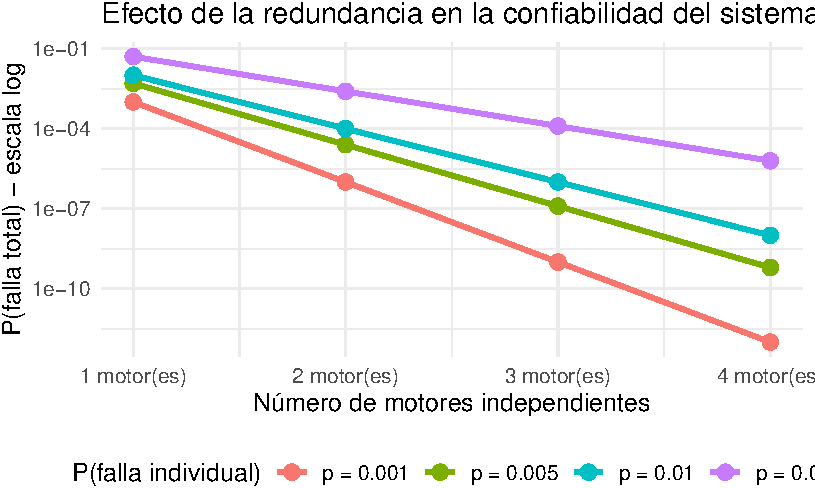
\includegraphics[keepaspectratio]{leccion-8-introduccion-a-la-probabilidad_files/figure-pdf/fig-redundancia-1.pdf}}

}

\caption{\label{fig-redundancia}Probabilidad de falla total del sistema
en escala logarítmica, en función del número de motores independientes,
para cuatro niveles de probabilidad individual de falla.}

\end{figure}%

Cada motor adicional reduce la probabilidad de falla total en varios
órdenes de magnitud. Este es el principio de diseño que hace que volar
sea una de las actividades más seguras del mundo moderno.

\textbf{Ejemplo adicional: independencia en una encuesta.} En una
encuesta a pilotos, el 10 \% son mujeres, el 30 \% vuela en aerolíneas
de bajo costo, y el 3 \% son mujeres que vuelan en bajo costo. ¿Son
independientes ``ser mujer'' y ``volar en bajo costo''?

\[P(\text{mujer}) \times P(\text{bajo costo}) = 0{,}10 \times 0{,}30 = 0{,}030 = P(\text{mujer y bajo costo}) \checkmark\]

La igualdad se verifica, de modo que ambos eventos son independientes en
esta muestra.

\begin{center}\rule{0.5\linewidth}{0.5pt}\end{center}

\section{Distribuciones de
probabilidad}\label{distribuciones-de-probabilidad}

Una \textbf{distribución de probabilidad} es una tabla o función que
lista todos los resultados disjuntos posibles de una variable aleatoria
junto con sus probabilidades. Toda distribución debe satisfacer tres
condiciones: los resultados son mutuamente excluyentes, cada
probabilidad está en \([0,1]\), y la suma de todas las probabilidades es
exactamente 1.

\subsection{Ejemplo clásico: suma de dos
dados}\label{ejemplo-cluxe1sico-suma-de-dos-dados}

La tabla siguiente muestra la distribución completa de la suma de dos
dados equilibrados.

{

\begin{longtable}[]{@{}cccc@{}}

\caption{\label{tbl-dados}Distribución de probabilidad para la suma de
dos dados. La suma de la columna Probabilidad es exactamente 1.}

\tabularnewline

\toprule\noalign{}
Suma & Casos favorables & Fracción & Probabilidad \\
\midrule\noalign{}
\endhead
\bottomrule\noalign{}
\endlastfoot
2 & 1 & 1/36 & 0.0278 \\
3 & 2 & 2/36 & 0.0556 \\
4 & 3 & 3/36 & 0.0833 \\
5 & 4 & 4/36 & 0.1111 \\
6 & 5 & 5/36 & 0.1389 \\
7 & 6 & 6/36 & 0.1667 \\
8 & 5 & 5/36 & 0.1389 \\
9 & 4 & 4/36 & 0.1111 \\
10 & 3 & 3/36 & 0.0833 \\
11 & 2 & 2/36 & 0.0556 \\
12 & 1 & 1/36 & 0.0278 \\

\end{longtable}

}

\begin{Shaded}
\begin{Highlighting}[]
\NormalTok{df\_dados }\OtherTok{\textless{}{-}} \FunctionTok{data.frame}\NormalTok{(}
  \AttributeTok{suma =} \DecValTok{2}\SpecialCharTok{:}\DecValTok{12}\NormalTok{,}
  \AttributeTok{prob =} \FunctionTok{c}\NormalTok{(}\DecValTok{1}\NormalTok{, }\DecValTok{2}\NormalTok{, }\DecValTok{3}\NormalTok{, }\DecValTok{4}\NormalTok{, }\DecValTok{5}\NormalTok{, }\DecValTok{6}\NormalTok{, }\DecValTok{5}\NormalTok{, }\DecValTok{4}\NormalTok{, }\DecValTok{3}\NormalTok{, }\DecValTok{2}\NormalTok{, }\DecValTok{1}\NormalTok{) }\SpecialCharTok{/} \DecValTok{36}
\NormalTok{)}

\FunctionTok{ggplot}\NormalTok{(df\_dados, }\FunctionTok{aes}\NormalTok{(}\AttributeTok{x =} \FunctionTok{as.factor}\NormalTok{(suma), }\AttributeTok{y =}\NormalTok{ prob)) }\SpecialCharTok{+}
  \FunctionTok{geom\_col}\NormalTok{(}\AttributeTok{fill =} \StringTok{"\#0758E5"}\NormalTok{, }\AttributeTok{color =} \StringTok{"white"}\NormalTok{, }\AttributeTok{width =} \FloatTok{0.75}\NormalTok{) }\SpecialCharTok{+}
  \FunctionTok{scale\_y\_continuous}\NormalTok{(}\AttributeTok{labels =} \FunctionTok{percent\_format}\NormalTok{(}\AttributeTok{accuracy =} \DecValTok{1}\NormalTok{)) }\SpecialCharTok{+}
  \FunctionTok{labs}\NormalTok{(}\AttributeTok{x =} \StringTok{"Suma de los dos dados"}\NormalTok{, }\AttributeTok{y =} \StringTok{"Probabilidad"}\NormalTok{,}
       \AttributeTok{title =} \StringTok{"Distribución de probabilidad — Suma de dos dados"}\NormalTok{) }\SpecialCharTok{+}
  \FunctionTok{theme\_minimal}\NormalTok{(}\AttributeTok{base\_size =} \DecValTok{12}\NormalTok{)}
\end{Highlighting}
\end{Shaded}

\begin{figure}[H]

\centering{

\pandocbounded{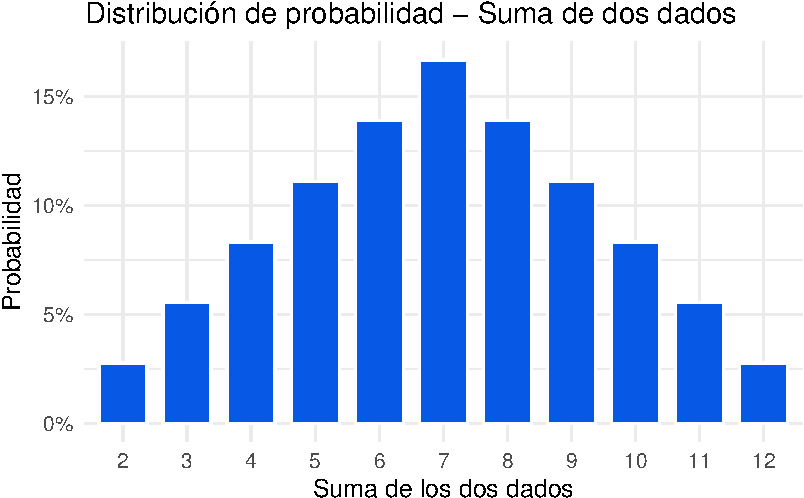
\includegraphics[keepaspectratio]{leccion-8-introduccion-a-la-probabilidad_files/figure-pdf/fig-dice-dist-1.pdf}}

}

\caption{\label{fig-dice-dist}Distribución de probabilidad de la suma de
dos dados. La forma triangular simétrica refleja que hay más maneras de
producir sumas intermedias que sumas extremas.}

\end{figure}%

\subsection{Aplicación aeronáutica: vuelos cancelados por
día}\label{aplicaciuxf3n-aeronuxe1utica-vuelos-cancelados-por-duxeda}

Según datos históricos de una aerolínea regional, la distribución del
número de vuelos cancelados en un día cualquiera es la siguiente. Puedes
verificar que \(0{,}60 + 0{,}25 + 0{,}10 + 0{,}04 + 0{,}01 = 1{,}00\).

\begin{Shaded}
\begin{Highlighting}[]
\NormalTok{df\_vuelos }\OtherTok{\textless{}{-}} \FunctionTok{data.frame}\NormalTok{(}
  \AttributeTok{x =} \DecValTok{0}\SpecialCharTok{:}\DecValTok{4}\NormalTok{,}
  \AttributeTok{p =} \FunctionTok{c}\NormalTok{(}\FloatTok{0.60}\NormalTok{, }\FloatTok{0.25}\NormalTok{, }\FloatTok{0.10}\NormalTok{, }\FloatTok{0.04}\NormalTok{, }\FloatTok{0.01}\NormalTok{)}
\NormalTok{)}

\FunctionTok{ggplot}\NormalTok{(df\_vuelos, }\FunctionTok{aes}\NormalTok{(}\AttributeTok{x =} \FunctionTok{factor}\NormalTok{(x), }\AttributeTok{y =}\NormalTok{ p)) }\SpecialCharTok{+}
  \FunctionTok{geom\_col}\NormalTok{(}\AttributeTok{fill =} \StringTok{"\#D7191C"}\NormalTok{, }\AttributeTok{color =} \StringTok{"white"}\NormalTok{, }\AttributeTok{width =} \FloatTok{0.65}\NormalTok{) }\SpecialCharTok{+}
  \FunctionTok{geom\_text}\NormalTok{(}\FunctionTok{aes}\NormalTok{(}\AttributeTok{label =} \FunctionTok{percent}\NormalTok{(p, }\AttributeTok{accuracy =} \DecValTok{1}\NormalTok{)),}
            \AttributeTok{vjust =} \SpecialCharTok{{-}}\FloatTok{0.5}\NormalTok{, }\AttributeTok{size =} \FloatTok{3.8}\NormalTok{) }\SpecialCharTok{+}
  \FunctionTok{scale\_y\_continuous}\NormalTok{(}\AttributeTok{labels =} \FunctionTok{percent\_format}\NormalTok{(}\AttributeTok{accuracy =} \DecValTok{1}\NormalTok{),}
                     \AttributeTok{limits =} \FunctionTok{c}\NormalTok{(}\DecValTok{0}\NormalTok{, }\FloatTok{0.68}\NormalTok{)) }\SpecialCharTok{+}
  \FunctionTok{labs}\NormalTok{(}\AttributeTok{x =} \StringTok{"Número de vuelos cancelados"}\NormalTok{, }\AttributeTok{y =} \StringTok{"Probabilidad"}\NormalTok{,}
       \AttributeTok{title =} \StringTok{"Distribución diaria de cancelaciones de vuelo"}\NormalTok{) }\SpecialCharTok{+}
  \FunctionTok{theme\_minimal}\NormalTok{(}\AttributeTok{base\_size =} \DecValTok{12}\NormalTok{)}
\end{Highlighting}
\end{Shaded}

\begin{figure}[H]

\centering{

\pandocbounded{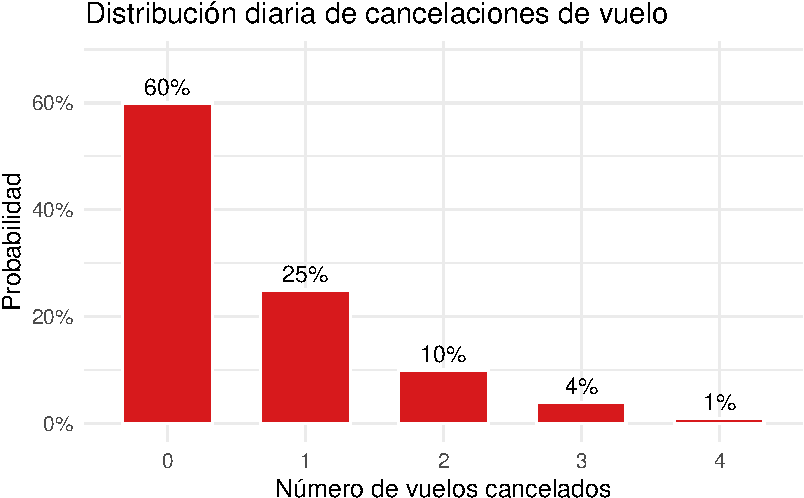
\includegraphics[keepaspectratio]{leccion-8-introduccion-a-la-probabilidad_files/figure-pdf/fig-vuelos-1.pdf}}

}

\caption{\label{fig-vuelos}Distribución de probabilidad para el número
de vuelos cancelados por día. El 60 \% de los días no se cancela ningún
vuelo.}

\end{figure}%

\begin{center}\rule{0.5\linewidth}{0.5pt}\end{center}

\section{Simulación en R: teoría y práctica frente a
frente}\label{simulaciuxf3n-en-r-teoruxeda-y-pruxe1ctica-frente-a-frente}

Una ventaja de R es que podemos simular procesos aleatorios y comparar
los resultados empíricos con las predicciones teóricas. El siguiente
código realiza 100.000 lanzamientos de dos dados y compara las
frecuencias relativas observadas con las probabilidades de la
distribución teórica.

\begin{Shaded}
\begin{Highlighting}[]
\FunctionTok{set.seed}\NormalTok{(}\DecValTok{2026}\NormalTok{)}
\NormalTok{n\_sim }\OtherTok{\textless{}{-}} \DecValTok{100000}

\CommentTok{\# Simulamos dos dados y calculamos su suma}
\NormalTok{dado1    }\OtherTok{\textless{}{-}} \FunctionTok{sample}\NormalTok{(}\DecValTok{1}\SpecialCharTok{:}\DecValTok{6}\NormalTok{, n\_sim, }\AttributeTok{replace =} \ConstantTok{TRUE}\NormalTok{)}
\NormalTok{dado2    }\OtherTok{\textless{}{-}} \FunctionTok{sample}\NormalTok{(}\DecValTok{1}\SpecialCharTok{:}\DecValTok{6}\NormalTok{, n\_sim, }\AttributeTok{replace =} \ConstantTok{TRUE}\NormalTok{)}
\NormalTok{suma\_sim }\OtherTok{\textless{}{-}}\NormalTok{ dado1 }\SpecialCharTok{+}\NormalTok{ dado2}

\CommentTok{\# Frecuencias relativas observadas}
\NormalTok{freq\_obs }\OtherTok{\textless{}{-}} \FunctionTok{as.data.frame}\NormalTok{(}\FunctionTok{table}\NormalTok{(suma\_sim) }\SpecialCharTok{/}\NormalTok{ n\_sim)}
\FunctionTok{names}\NormalTok{(freq\_obs) }\OtherTok{\textless{}{-}} \FunctionTok{c}\NormalTok{(}\StringTok{"suma"}\NormalTok{, }\StringTok{"freq\_obs"}\NormalTok{)}
\NormalTok{freq\_obs}\SpecialCharTok{$}\NormalTok{suma   }\OtherTok{\textless{}{-}} \FunctionTok{as.integer}\NormalTok{(}\FunctionTok{as.character}\NormalTok{(freq\_obs}\SpecialCharTok{$}\NormalTok{suma))}

\CommentTok{\# Probabilidades teóricas}
\NormalTok{df\_teo }\OtherTok{\textless{}{-}} \FunctionTok{data.frame}\NormalTok{(}
  \AttributeTok{suma     =} \DecValTok{2}\SpecialCharTok{:}\DecValTok{12}\NormalTok{,}
  \AttributeTok{prob\_teo =} \FunctionTok{c}\NormalTok{(}\DecValTok{1}\NormalTok{, }\DecValTok{2}\NormalTok{, }\DecValTok{3}\NormalTok{, }\DecValTok{4}\NormalTok{, }\DecValTok{5}\NormalTok{, }\DecValTok{6}\NormalTok{, }\DecValTok{5}\NormalTok{, }\DecValTok{4}\NormalTok{, }\DecValTok{3}\NormalTok{, }\DecValTok{2}\NormalTok{, }\DecValTok{1}\NormalTok{) }\SpecialCharTok{/} \DecValTok{36}
\NormalTok{)}

\CommentTok{\# Fusionamos y pasamos a formato largo para ggplot}
\NormalTok{df\_comp }\OtherTok{\textless{}{-}} \FunctionTok{merge}\NormalTok{(df\_teo, freq\_obs, }\AttributeTok{by =} \StringTok{"suma"}\NormalTok{) }\SpecialCharTok{|\textgreater{}}
  \FunctionTok{pivot\_longer}\NormalTok{(}\AttributeTok{cols =} \FunctionTok{c}\NormalTok{(}\StringTok{"prob\_teo"}\NormalTok{, }\StringTok{"freq\_obs"}\NormalTok{),}
               \AttributeTok{names\_to =} \StringTok{"tipo"}\NormalTok{, }\AttributeTok{values\_to =} \StringTok{"valor"}\NormalTok{) }\SpecialCharTok{|\textgreater{}}
  \FunctionTok{mutate}\NormalTok{(}\AttributeTok{tipo =} \FunctionTok{ifelse}\NormalTok{(tipo }\SpecialCharTok{==} \StringTok{"prob\_teo"}\NormalTok{, }\StringTok{"Teórica"}\NormalTok{, }\StringTok{"Simulada"}\NormalTok{))}

\FunctionTok{ggplot}\NormalTok{(df\_comp, }\FunctionTok{aes}\NormalTok{(}\AttributeTok{x =}\NormalTok{ suma, }\AttributeTok{y =}\NormalTok{ valor, }\AttributeTok{fill =}\NormalTok{ tipo)) }\SpecialCharTok{+}
  \FunctionTok{geom\_col}\NormalTok{(}\AttributeTok{position =} \StringTok{"dodge"}\NormalTok{, }\AttributeTok{width =} \FloatTok{0.75}\NormalTok{, }\AttributeTok{color =} \StringTok{"white"}\NormalTok{) }\SpecialCharTok{+}
  \FunctionTok{scale\_x\_continuous}\NormalTok{(}\AttributeTok{breaks =} \DecValTok{2}\SpecialCharTok{:}\DecValTok{12}\NormalTok{) }\SpecialCharTok{+}
  \FunctionTok{scale\_y\_continuous}\NormalTok{(}\AttributeTok{labels =} \FunctionTok{percent\_format}\NormalTok{(}\AttributeTok{accuracy =} \DecValTok{1}\NormalTok{)) }\SpecialCharTok{+}
  \FunctionTok{scale\_fill\_manual}\NormalTok{(}\AttributeTok{values =} \FunctionTok{c}\NormalTok{(}\StringTok{"Teórica"} \OtherTok{=} \StringTok{"\#0758E5"}\NormalTok{,}
                               \StringTok{"Simulada"} \OtherTok{=} \StringTok{"\#FDAE61"}\NormalTok{)) }\SpecialCharTok{+}
  \FunctionTok{labs}\NormalTok{(}\AttributeTok{x =} \StringTok{"Suma de dos dados"}\NormalTok{,}
       \AttributeTok{y =} \StringTok{"Probabilidad / Frecuencia relativa"}\NormalTok{,}
       \AttributeTok{fill =} \StringTok{""}\NormalTok{,}
       \AttributeTok{title =} \StringTok{"Probabilidad teórica vs. simulación (n = 100.000)"}\NormalTok{) }\SpecialCharTok{+}
  \FunctionTok{theme\_minimal}\NormalTok{(}\AttributeTok{base\_size =} \DecValTok{12}\NormalTok{) }\SpecialCharTok{+}
  \FunctionTok{theme}\NormalTok{(}\AttributeTok{legend.position =} \StringTok{"bottom"}\NormalTok{)}
\end{Highlighting}
\end{Shaded}

\begin{figure}[H]

\centering{

\pandocbounded{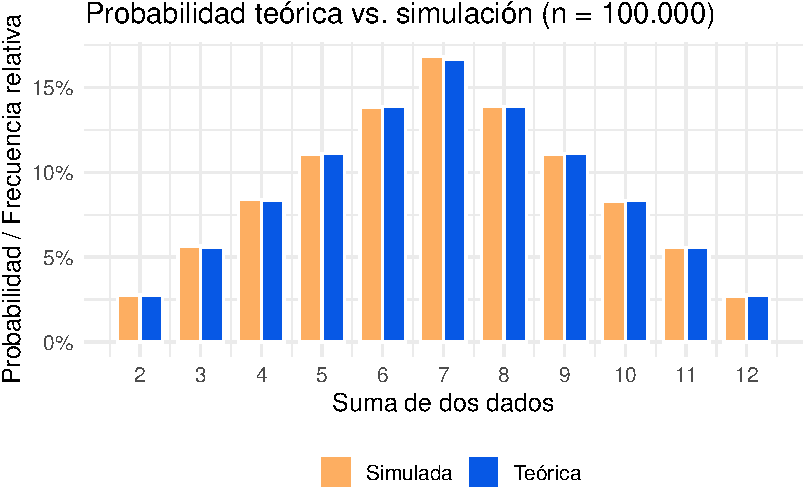
\includegraphics[keepaspectratio]{leccion-8-introduccion-a-la-probabilidad_files/figure-pdf/fig-sim-comparacion-1.pdf}}

}

\caption{\label{fig-sim-comparacion}Comparación entre probabilidades
teóricas (azul) y frecuencias simuladas (naranja) para la suma de dos
dados con n = 100.000 lanzamientos. La Ley de los Grandes Números
garantiza el estrecho acuerdo entre ambas.}

\end{figure}%

El acuerdo entre ambas distribuciones es muy estrecho, y cualquier
diferencia residual se debe al azar de la simulación. Si repitieras con
\(n = 10^6\), las diferencias serían aún menores.

\begin{center}\rule{0.5\linewidth}{0.5pt}\end{center}

\section{Síntesis de conceptos
clave}\label{suxedntesis-de-conceptos-clave}

La siguiente tabla resume las reglas fundamentales desarrolladas a lo
largo de la lección.

{\def\LTcaptype{none} % do not increment counter
\begin{longtable}[]{@{}
  >{\raggedright\arraybackslash}p{(\linewidth - 4\tabcolsep) * \real{0.3333}}
  >{\raggedright\arraybackslash}p{(\linewidth - 4\tabcolsep) * \real{0.3333}}
  >{\raggedright\arraybackslash}p{(\linewidth - 4\tabcolsep) * \real{0.3333}}@{}}
\toprule\noalign{}
\begin{minipage}[b]{\linewidth}\raggedright
Concepto
\end{minipage} & \begin{minipage}[b]{\linewidth}\raggedright
Expresión matemática
\end{minipage} & \begin{minipage}[b]{\linewidth}\raggedright
Condición de aplicación
\end{minipage} \\
\midrule\noalign{}
\endhead
\bottomrule\noalign{}
\endlastfoot
Espacio muestral completo & \(P(S) = 1\) & Siempre \\
Evento imposible & \(P(\emptyset) = 0\) & Siempre \\
Complemento & \(P(A^c) = 1 - P(A)\) & Siempre \\
Adición (disjuntos) & \(P(A \cup B) = P(A) + P(B)\) &
\(A \cap B = \emptyset\) \\
Adición (general) & \(P(A \cup B) = P(A) + P(B) - P(A \cap B)\) &
Siempre \\
Multiplicación & \(P(A \cap B) = P(A) \cdot P(B)\) & \(A\) y \(B\)
independientes \\
\end{longtable}
}

\begin{center}\rule{0.5\linewidth}{0.5pt}\end{center}

\section{Cuestionario grupal}\label{cuestionario-grupal}

Responde las siguientes preguntas mostrando el razonamiento y los
cálculos necesarios. Cuando corresponda, indica qué regla estás
aplicando y por qué es válida en ese contexto.

\textbf{Pregunta 1 --- Dados y eventos.} Al lanzar un dado equilibrado
de seis caras: (a) ¿Cuál es la probabilidad de obtener un número mayor
que 4? (b) ¿Cuál es la probabilidad de obtener un número impar o un 6?
(c) ¿Son los eventos ``obtener un número par'' y ``obtener un número
mayor que 3'' disjuntos? Justifica con el espacio muestral.

\textbf{Pregunta 2 --- Cartas.} De un mazo estándar de 52 cartas se
extrae una carta al azar. Calcula: (a) la probabilidad de que sea un as;
(b) la probabilidad de que sea un as o una carta de tréboles; (c) la
probabilidad de que no sea un as.

\textbf{Pregunta 3 --- Vuelos cancelados.} En cierto aeropuerto,
\(P(\text{cancelación por mal tiempo}) = 0{,}02\),
\(P(\text{cancelación por problemas técnicos}) = 0{,}01\), y
\(P(\text{ambas causas}) = 0{,}002\). (a) ¿Son disjuntos estos eventos?
Explica. (b) Calcula la probabilidad de cancelación por una u otra
causa. (c) Si la probabilidad de que un vuelo salga a tiempo es
\(0{,}85\), ¿cuál es la probabilidad de que se retrase o cancele?

\textbf{Pregunta 4 --- Motores de avión.} Un avión de cuatro motores
puede volar si al menos dos funcionan. Cada motor tiene probabilidad de
falla independiente \(p = 0{,}002\). (a) Calcula la probabilidad de que
los cuatro motores funcionen correctamente. (b) Calcula la probabilidad
de que exactamente un motor falle. (c) ¿Es el sistema de cuatro motores
más seguro que un bimotor con los mismos motores? Justifica
cuantitativamente.

\textbf{Pregunta 5 --- Simulación con R.} Modifica el código de la
lección para estimar la probabilidad de obtener un 6 al lanzar un dado.
(a) ¿Cuál es la probabilidad teórica? (b) Realiza la simulación con
\(n = 1{.}000\) y \(n = 100{.}000\) lanzamientos. ¿Qué diferencias
observas en la precisión? Relaciona tu respuesta con la Ley de los
Grandes Números.

\textbf{Pregunta 6 --- Independencia.} En una encuesta a pilotos, el 10
\% son mujeres, el 30 \% vuela en aerolíneas de bajo costo, y el 3 \%
son mujeres que vuelan en bajo costo. ¿Son los eventos ``ser mujer'' y
``volar en bajo costo'' independientes? Muestra los cálculos y expresa
la conclusión en palabras.

\begin{center}\rule{0.5\linewidth}{0.5pt}\end{center}

¡Sigue practicando! La probabilidad es el lenguaje de la incertidumbre,
y dominarlo te permitirá entender, construir y cuestionar con rigor
cualquier afirmación basada en datos. Cualquier duda, consulta con el
profesor.

\emph{Prof.~Hans Sigrist --- Colegio Portaliano, San Felipe}




\end{document}
